An important part of this work is a toolchain embodying the methodology. The
toolchain has been implemented in the Rust programming language
\cite{rust}.\footnote{Rust is a systems programming developed by Mozilla
Research and thousands of independent contributors from all around the world.
Rust focuses on memory safety without garbage collection, concurrency without
data races, abstractions without overhead, and stability without stagnation.} It
consists of a number of command-line tools, and the tools are composed of a
number of stand-alone packages. The toolchain also makes use of third-party
software, including the state-of-the-art simulators introduced in
\sref{prior-work}. Regardless of the origin, each component toolchain is open
source. The code written by us is distributed under the \sc{MIT} license
\cite{mit} and is available at \cite{sources}.

The main programs of our toolchain are called Recorder and Streamer, and we
shall describe their architectures next.

\subsection{Recorder}
\begin{figure}
  \centering
  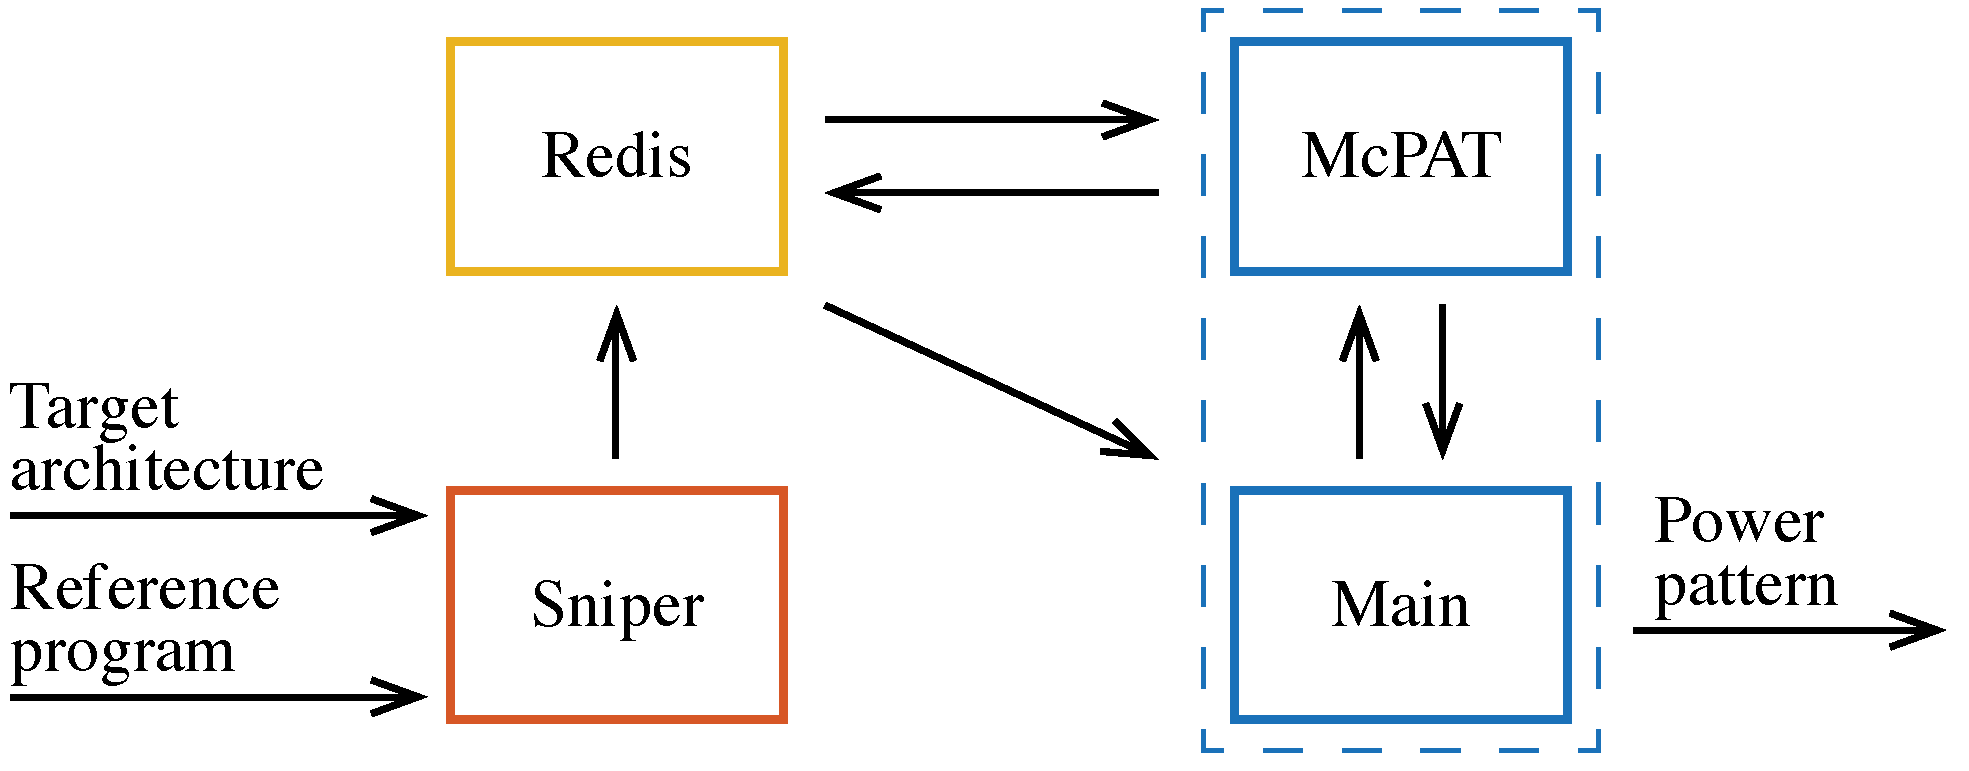
\includegraphics[width=1.0\columnwidth]{include/assets/figures/recorder.pdf}
  \caption{The recording infrastructure.}
  \flab{recorder}
\end{figure}

As the name suggests, the purpose of \recorder\ is recording. More specifically,
the tool records power traces, which are needed as an input to \streamer. The
recording infrastructure is depicted in \fref{recorder}.

Sniper \cite{carlson2011}.
\begin{table}
  \caption{Target architecture}
  \begin{tabular*}{\linewidth}{=L{70pt}l}
    \toprule
    Component    & Description \\
    \midrule
    Core         & 2660 MHz, 1.2 V \\
    L1-I/D cache & 32 KB, 4-way, LRU, private \\
    L2 cache     & 256 KB, 4-way, LRU, private \\
    L3 cache     & 8192 KB, 16-way, LRU, one per four cores \\
    \bottomrule
  \end{tabular*}
  \tlab{target}
\end{table}
% vim: nowrap tw=0


The key-value storage is Redis \cite{redis}. The database is SQLite
\cite{sqlite}.

\sc{McPAT} \cite{li2009}.


\subsection{Streamer}
\begin{figure}
  \centering
  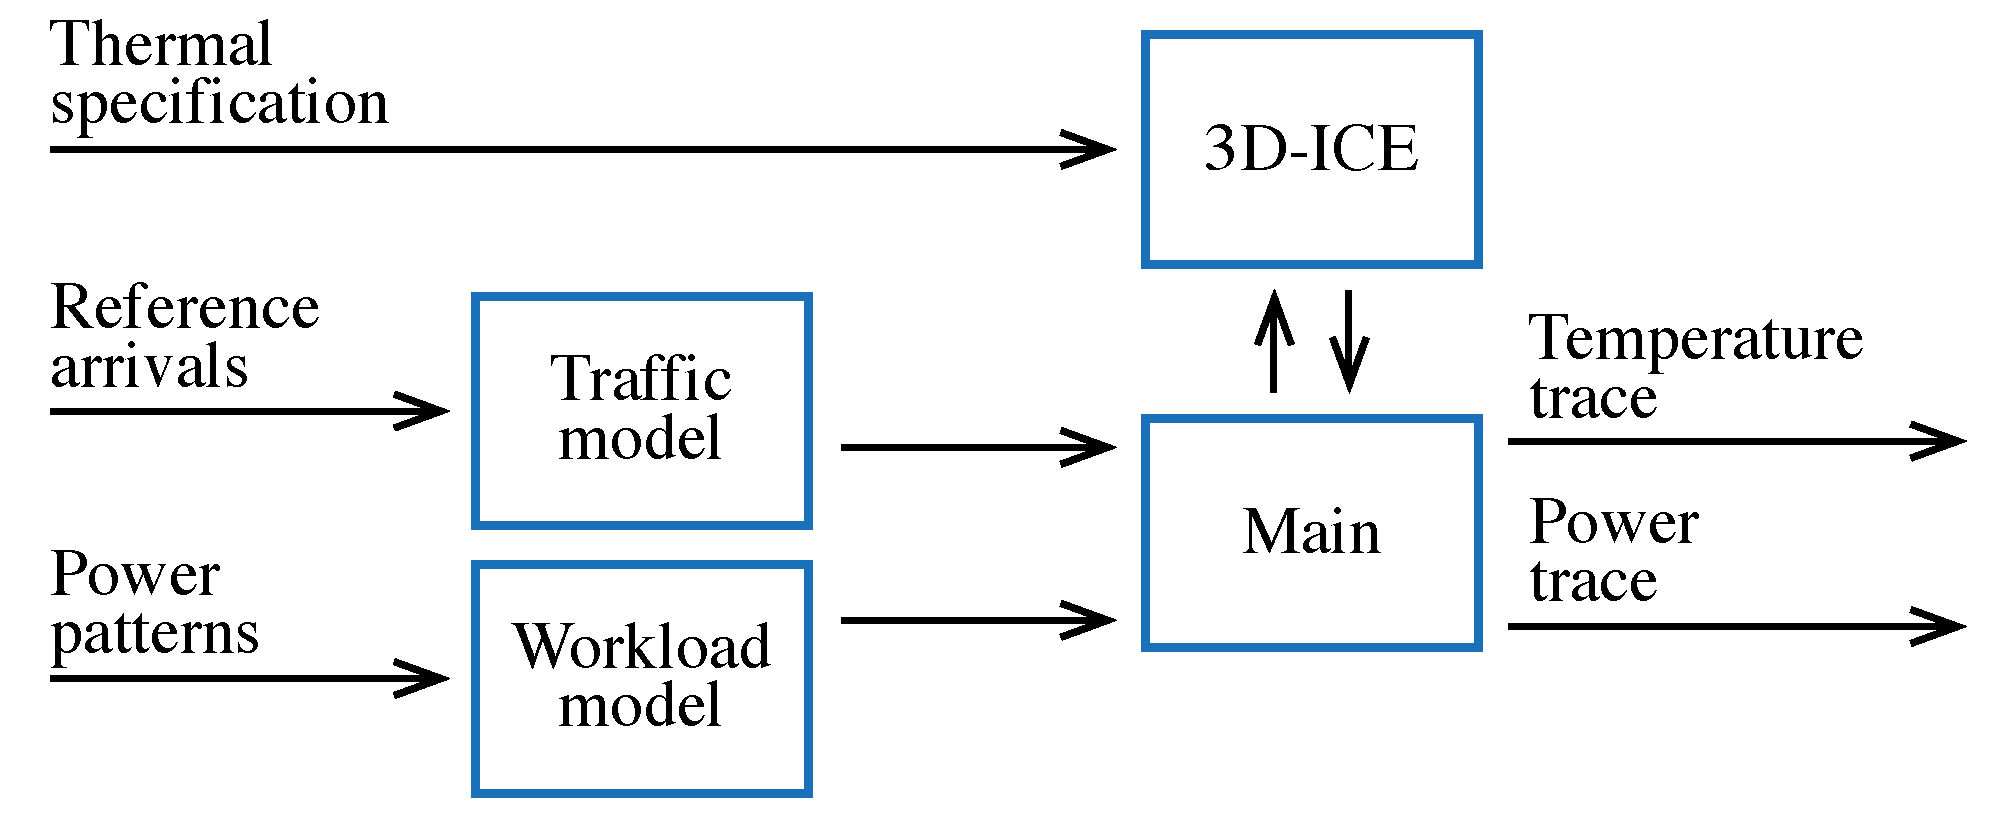
\includegraphics[width=1.0\columnwidth]{include/assets/figures/streamer.pdf}
  \caption{The streaming infrastructure.}
  \flab{streamer}
\end{figure}

The streaming infrastructure is depicted in \fref{streamer}.

HotSpot \cite{skadron2004}.
\sc{3D-ICE} \cite{sridhar2010}.
The solver is based on exponential integrators \cite{hochbruck2010},
\cite{ukhov2012}.

